%----------------------------------------------------------------------------
\chapter{Own work}\label{ch:own-work}
%----------------------------------------------------------------------------

In this chapter, I will describe my work, from the specification of the task through the testing process to the results. The structuring of the experiments will mostly follow a chronological timeline, with the most basic questions answered first.

\section{Defining the objective}\label{sec:defining-the-objective}

The first problem I encountered during my work was that there is no clear definition of what a good embedding is. No simple metric exists that accurately and fully captures the nuances of embedding a latent chemical space in lower dimension. This is not surprising, since the very existence of so many different dimension algorithms comes from the fact that there is no consensus on that a good dimension reduction algorithm does. As such, I needed to define my own metrics for ranking each embedding. For this, I turned to the underlying goal of embedding these molecules.

The main objective of my thesis is exploring the capability of the previously described dimension reduction algorithms in novel drug discovery. Some assumptions must be made for formalizing the requirements. The first such assumption is that molecules that have similar a structure also have similar chemical properties. While this statement is not true for all chemical descriptors, it holds for most non-categorical metrics, such as number of rings in the molecule, or the topological polar surface area (TPSA~\cite{bib:tpsa}). This intuition implies that molecules with similar structure have similar binding properties to certain proteins too, which is the most vital metric for novel drug research. Drug molecules act by binding to proteins, forming complexes that induce physiological changes in the body. The efficacy of binding depends on the chemical properties of the target protein (mainly its three-dimensional shape) and the chemical properties of the drug molecule.

From this, it logically follows that a chemical space that is ordered over the chemical structure of molecules allows the targeted search of potential drug candidates. Unfortunately, chemical structure can not be quantized in such a way as to be able to order them. Instead, I decided that what I needed was a space that \textit{smooth} over chemical structure. In essence, this means that points close to each other have similar chemical structure. This is the exact property that is needed for targeted search. Importantly, this does not imply that points far away from each other have significantly different structure. Optimizing for embedding all similar molecules closely is a difficult task, and I can not be sure that points in the original 64-dimensional dataset even satisfies this condition. An algorithm that places all similarly structured molecules close together is advantageous, but for my purposes, not needed.

In summary, a good embedding is one that is locally smooth over chemical structure. This can most easily be determined by looking at chemical descriptors of molecules, and assessing their local smoothness in the output space.

The choice of descriptors matters greatly in this question. The original model was trained on millions of molecules, and some of their chemical properties. The properties used by the VAE's property predictor was part of the database, which means that the 64-dimensional latent space should in theory be relatively smooth over those metrics. Because of this, the inclusion of other chemical descriptors are needed for a proper examination of data. With mostly smooth transitions on a large number of descriptors, one can be certain that the chemical structure itself changes smoothly.

\section{Initial testing}\label{sec:initial-testing}

After defining the objective, the first thing that I did was running each algorithm with default parametrization to see baseline results. This served two purposes. Firstly, by generating baseline embeddings, the effect of different parametrization could be more accurately assessed. Secondly, I recorded the runtime of each algorithm, so their performance could be compared from a different angle.

After running each algorithm once, I noticed that the t-SNE clustering was somewhat strange (as can be seen on figure (\ref{fig:default_run})). The result of this run did not make much sense. It was completely different from what I expected. I had prior experience using t-SNE, albeit another implementation. After rerunning the algorithm, I found a similar result, which led me to believe that the implementation had some bug. Indeed, when I ran t-SNE again in verbose mode, I found that instead of the 2000 iterations specified, it only ran for about 150, which was not enough to form proper clusters. I tried switching to openTSNE, the implementation I used heavily during my project laboratory, however, the sheer size of the dataset made it unusable as the system did not have enough memory to accommodate its needs.

After some consideration, I turned to tsnecuda, another familiar implementation that ran on the GPU (and as such, used its own memory instead of the RAM of the system). I initially chose openTSNE for two reasons: firstly, it was more usable that tsnecuda, as it was far more parametrizable, allowing for custom callback functions and deterministic runs. Secondly, all other algorithm ran on the CPU, making performance comparisons more fair with openTSNE. Since openTSNE could not even complete one run, I was forced to use tsnecuda. This switch however highlighted something very interesting.

In the field of deep learning, GPU's are widely used as they are capable of running thousands of operations in parallel, leading to faster training of models. All graph-based clustering algorithms work very similarly to a neural network, in that they exclusively work with matrices and are highly parallelizable. This means that using GPU resources can significantly speed up the clustering of any given dataset. As can be seen on table (\ref{tab:runtime}), while the sklearn t-SNE implementation took almost exactly 25 hours to run for 150 iterations (plus constructing the higher dimensional probability distribution), tsnecuda did not even take six minutes to perform 5000 iterations (in fact, in the first run, I set it to only 2000 iterations, which ran for 102 seconds, an incredible 883 times faster).

\begin{table}[htb]
	\begin{center}
		\begin{tabular}{|l|r|}
			\hline
			Algorithm (iterations) & runtime \\
			\hline
			PCA & 19.45 s \\
			\hline
			t-SNE (sklearn, 150) & 90 042 s \\
			\hline
			t-SNE (tsnecuda, 5000) & 344.29 s \\
			\hline
			UMAP (1000 epochs) & 5 866.55 s \\
			\hline
			TriMAP (2000) & 26 756.64 s \\
			\hline
			PaCMAP (2000) & 65 283.52 s \\
			\hline
		\end{tabular}
	\end{center}
	\caption{Runtimes of each algorithm tested on the entire dataset (without duplicates, ~1.6 million molecules) given in seconds. The number of iterations and epochs are indicated where applicable. PCA, the only non-iterative method is the fastest, while the others take significantly more time. The power of GPU usage is clearly demonstrated by the two t-SNE implementations.}
	\label{tab:runtime}
\end{table}

Comparison of each algorithm based on the runtimes in table (\ref{tab:runtime}) should only be done in context. PCA is the fastest method of the bunch, this is because it is the only non-iterative algorithm. After that, the GPU implementation of t-SNE is the fastest, but this can not be credited to the algorithm, but the implementation instead. In fact, the slowest running algorithm is also a t-SNE implementation, which ran on the CPU. As for the other graph-based algorithms, they are not equal either. UMAP has multithreaded capabilities, while TriMAP and PaCMAP do not.

In summary, these runtime metrics are not intrinsic properties of the algorithms. They merely describe the performance of the current implementations. In time, more libraries will be available for every algorithm and these numbers will change. t-SNE and UMAP both have GPU implementations which vastly outperform their CPU implementations, and even other algorithms that are supposed to be faster than them. In an engineering application, it is important to consider technical parameters, it should be noted that these parameters change as opposed to each algorithm's performance in terms of the quality of the embedding.

\section{Result of first runs}\label{sec:result-of-first-runs}

I have briefly touched on the importance of chemical descriptors in the inference of structure in section (\ref{sec:defining-the-objective}). Since the original model was trained with a property predictor, it is to be expected that the latent space is smooth over those descriptors. This can be seen on figure (\ref{fig:default_run}) with the quantitative estimate of drug-likeness (qed~\cite{bib:qed}). Additional metrics were needed to properly be able to induce chemical structure. This is needed because while structural similarity between molecules can easily be captured by one number, the structure of individual molecules is typically described by fingerprint vectors. These would form a vector space that is not easy to interpret.

\begin{figure}[!ht]
	\centering
	\includegraphics[width=0.49\columnwidth, keepaspectratio]{figures/PCA_default}
	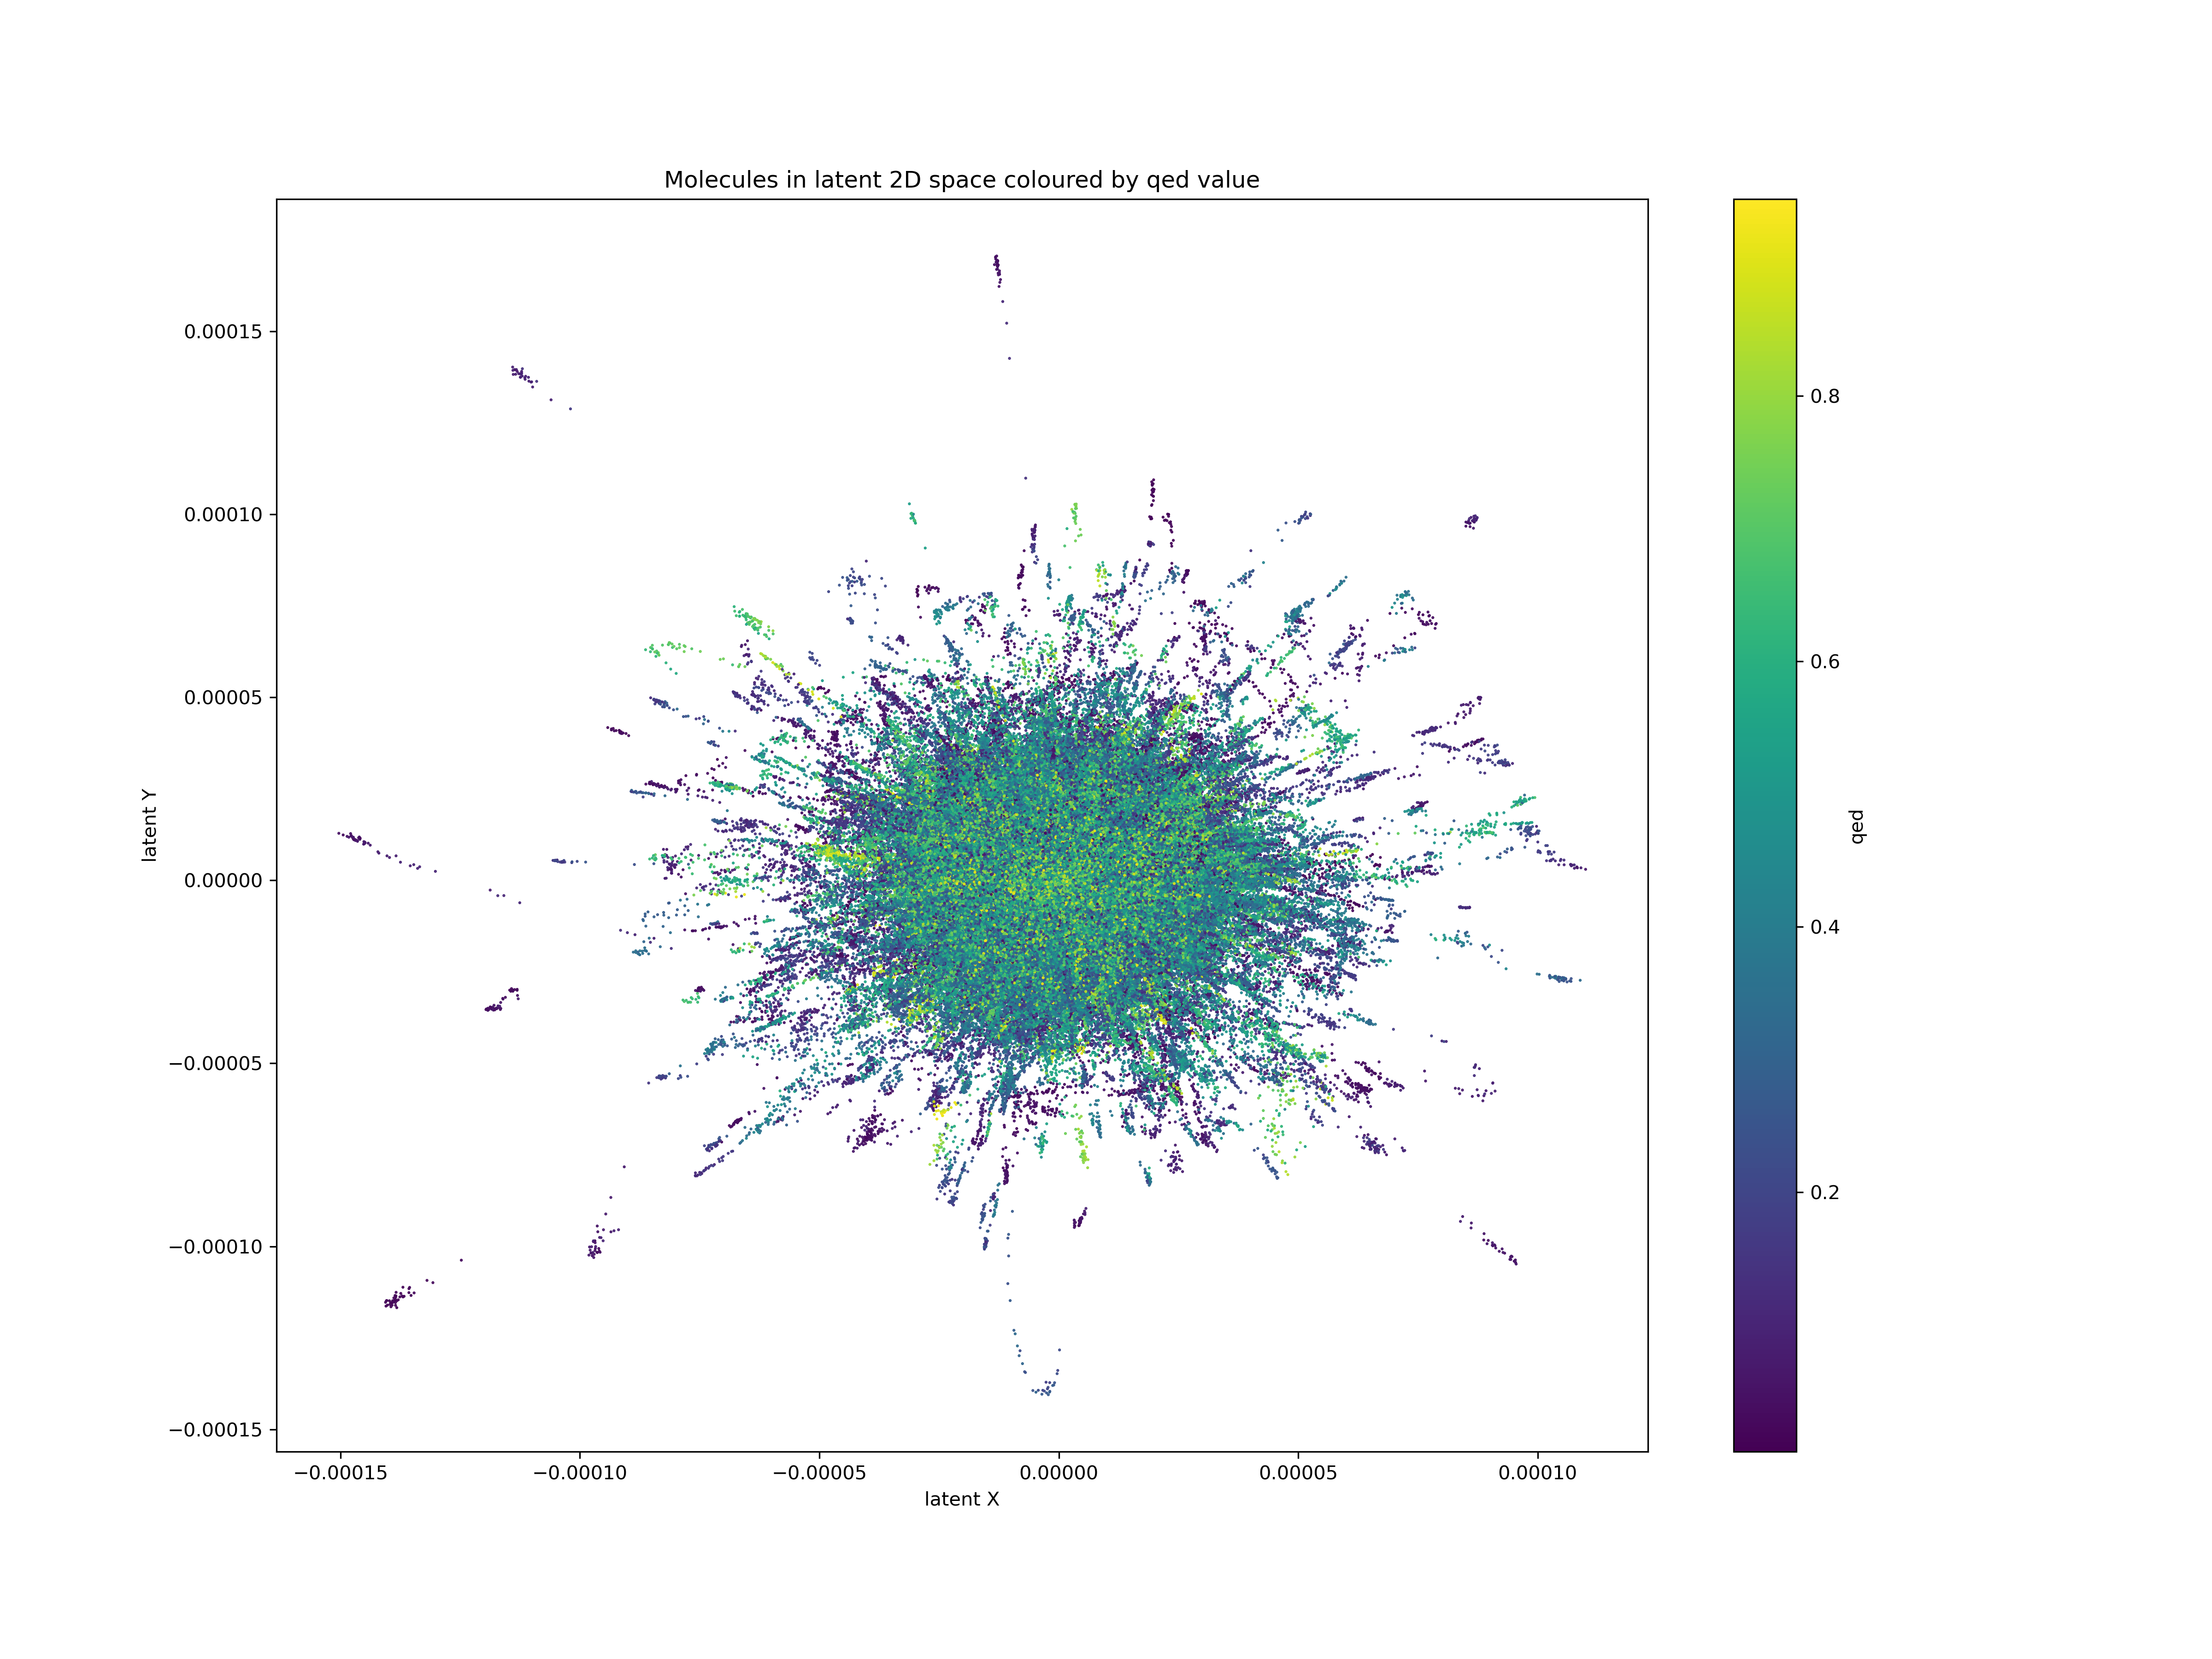
\includegraphics[width=0.49\columnwidth, keepaspectratio]{figures/t-SNE_default}
	\includegraphics[width=0.49\columnwidth, keepaspectratio]{figures/t-SNE2_default}
	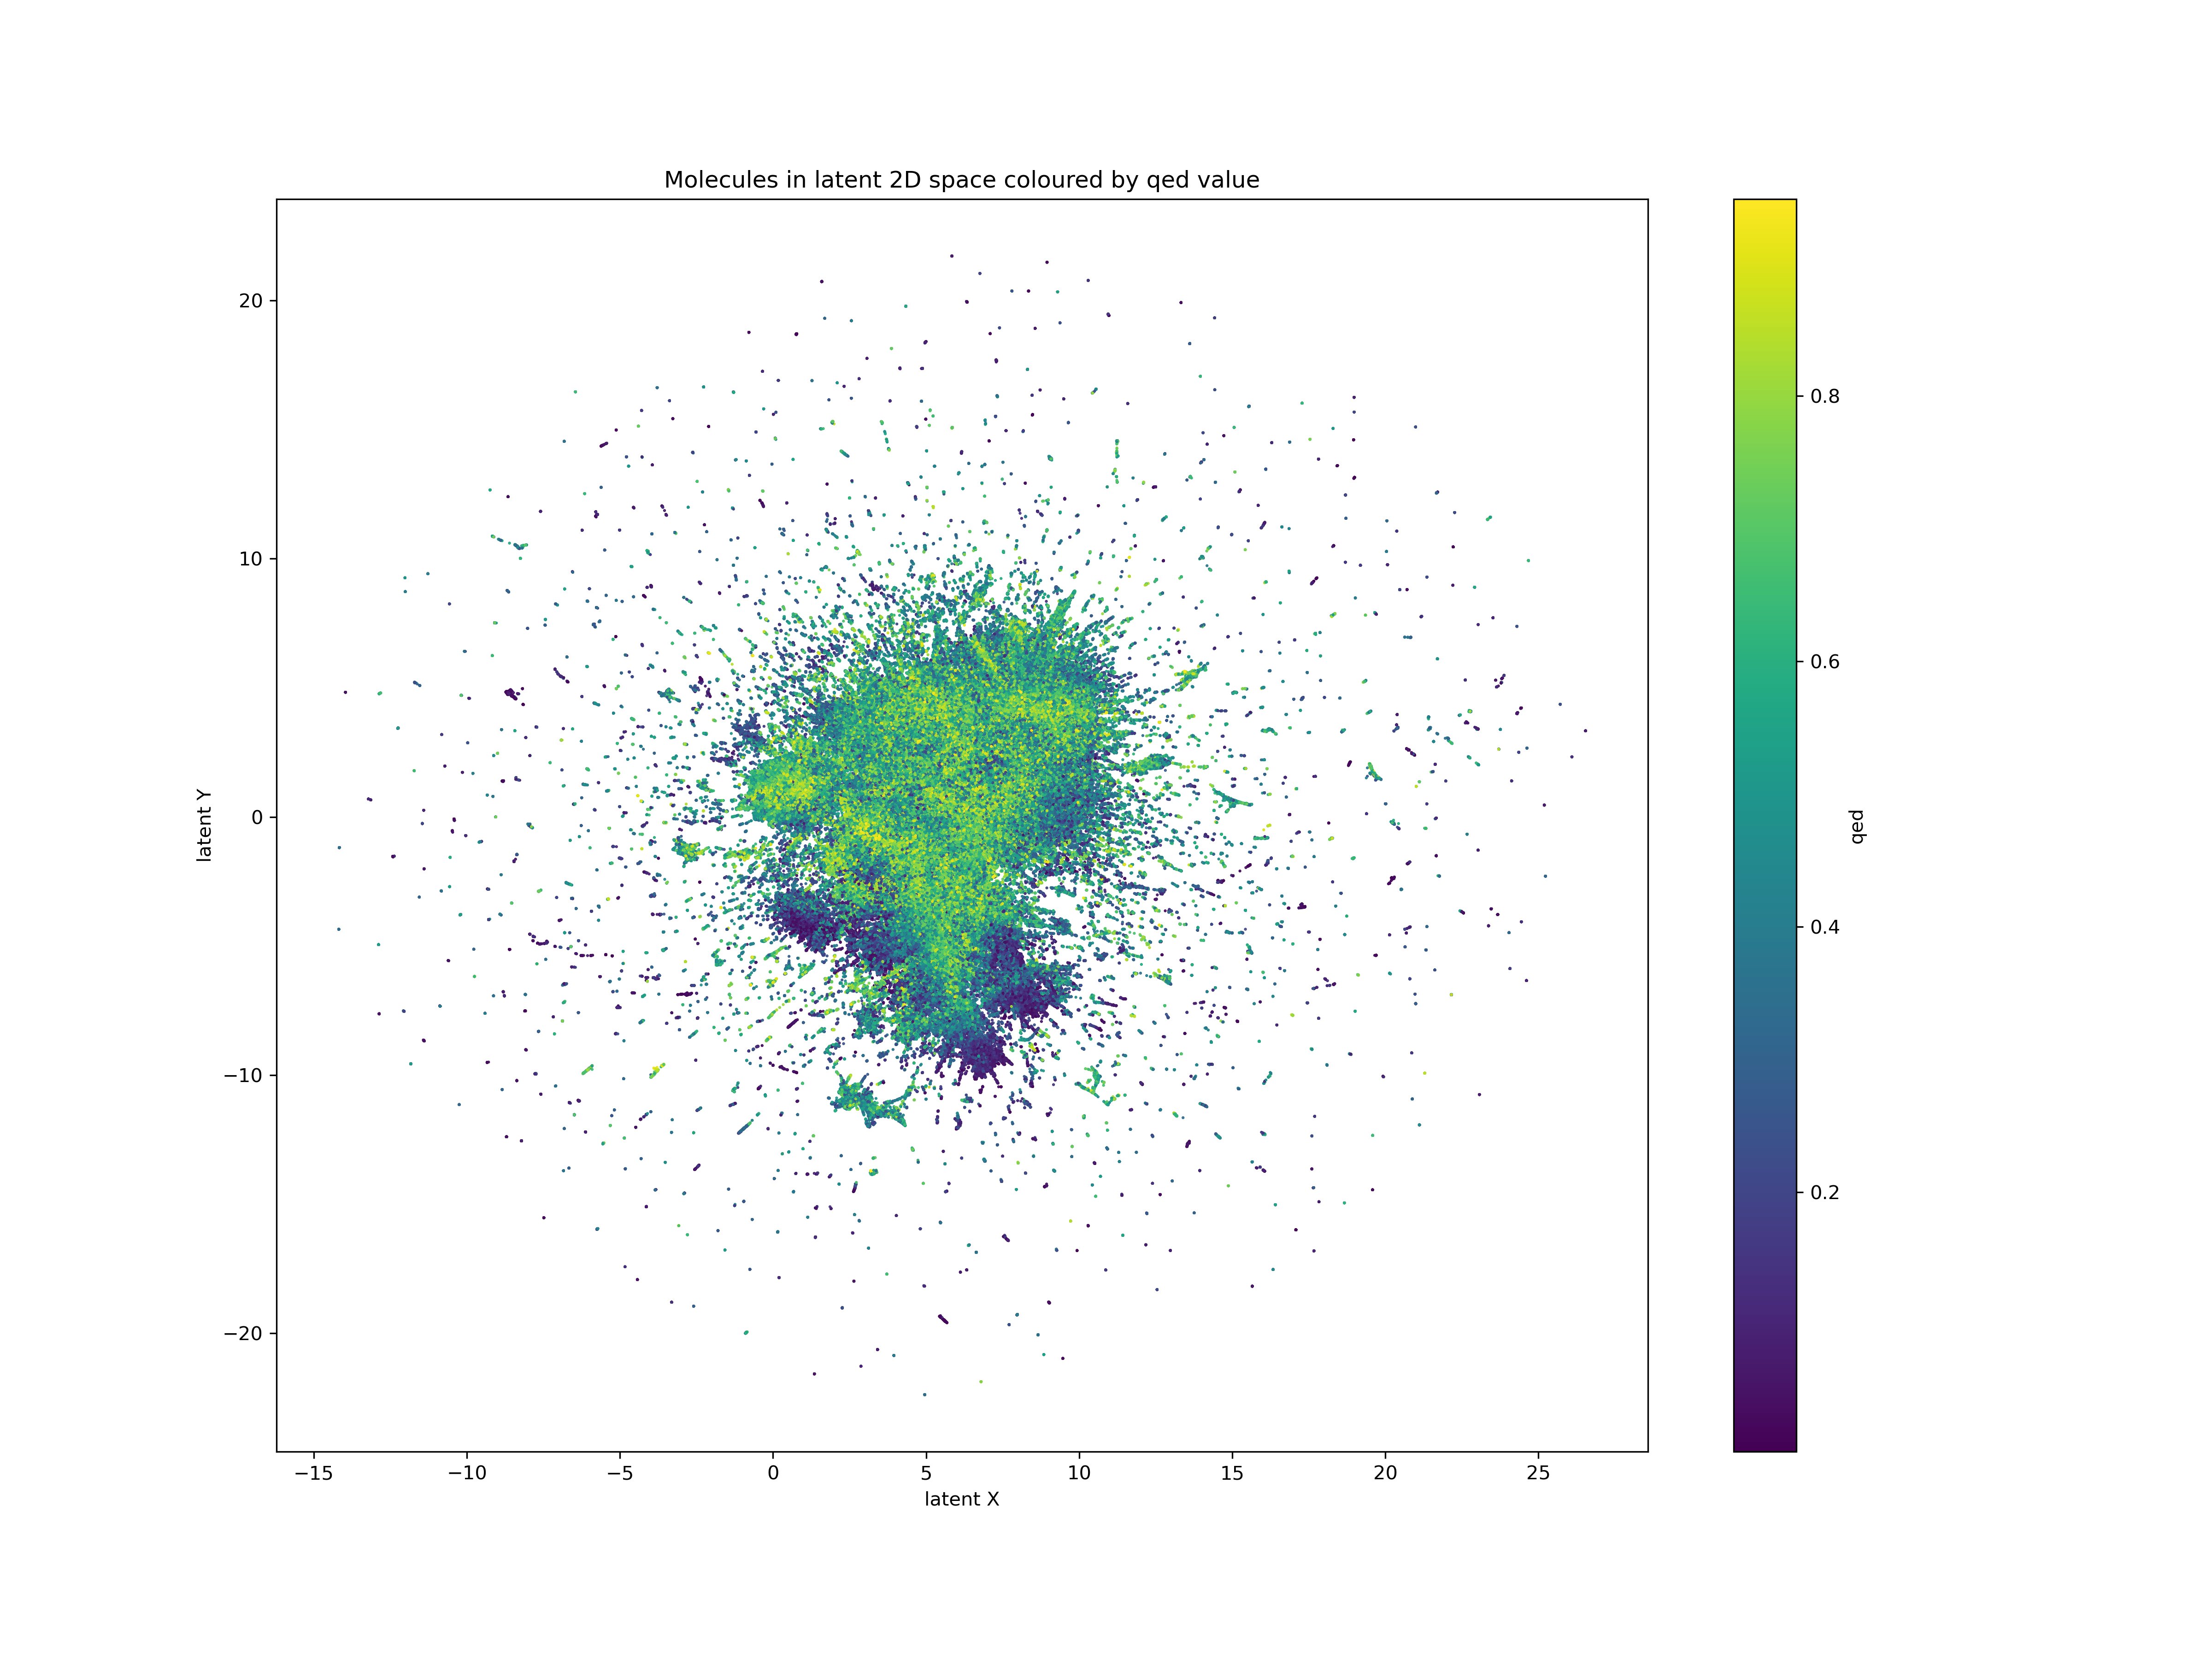
\includegraphics[width=0.49\columnwidth, keepaspectratio]{figures/UMAP_default}
	\includegraphics[width=0.49\columnwidth, keepaspectratio]{figures/TriMAP_default}
	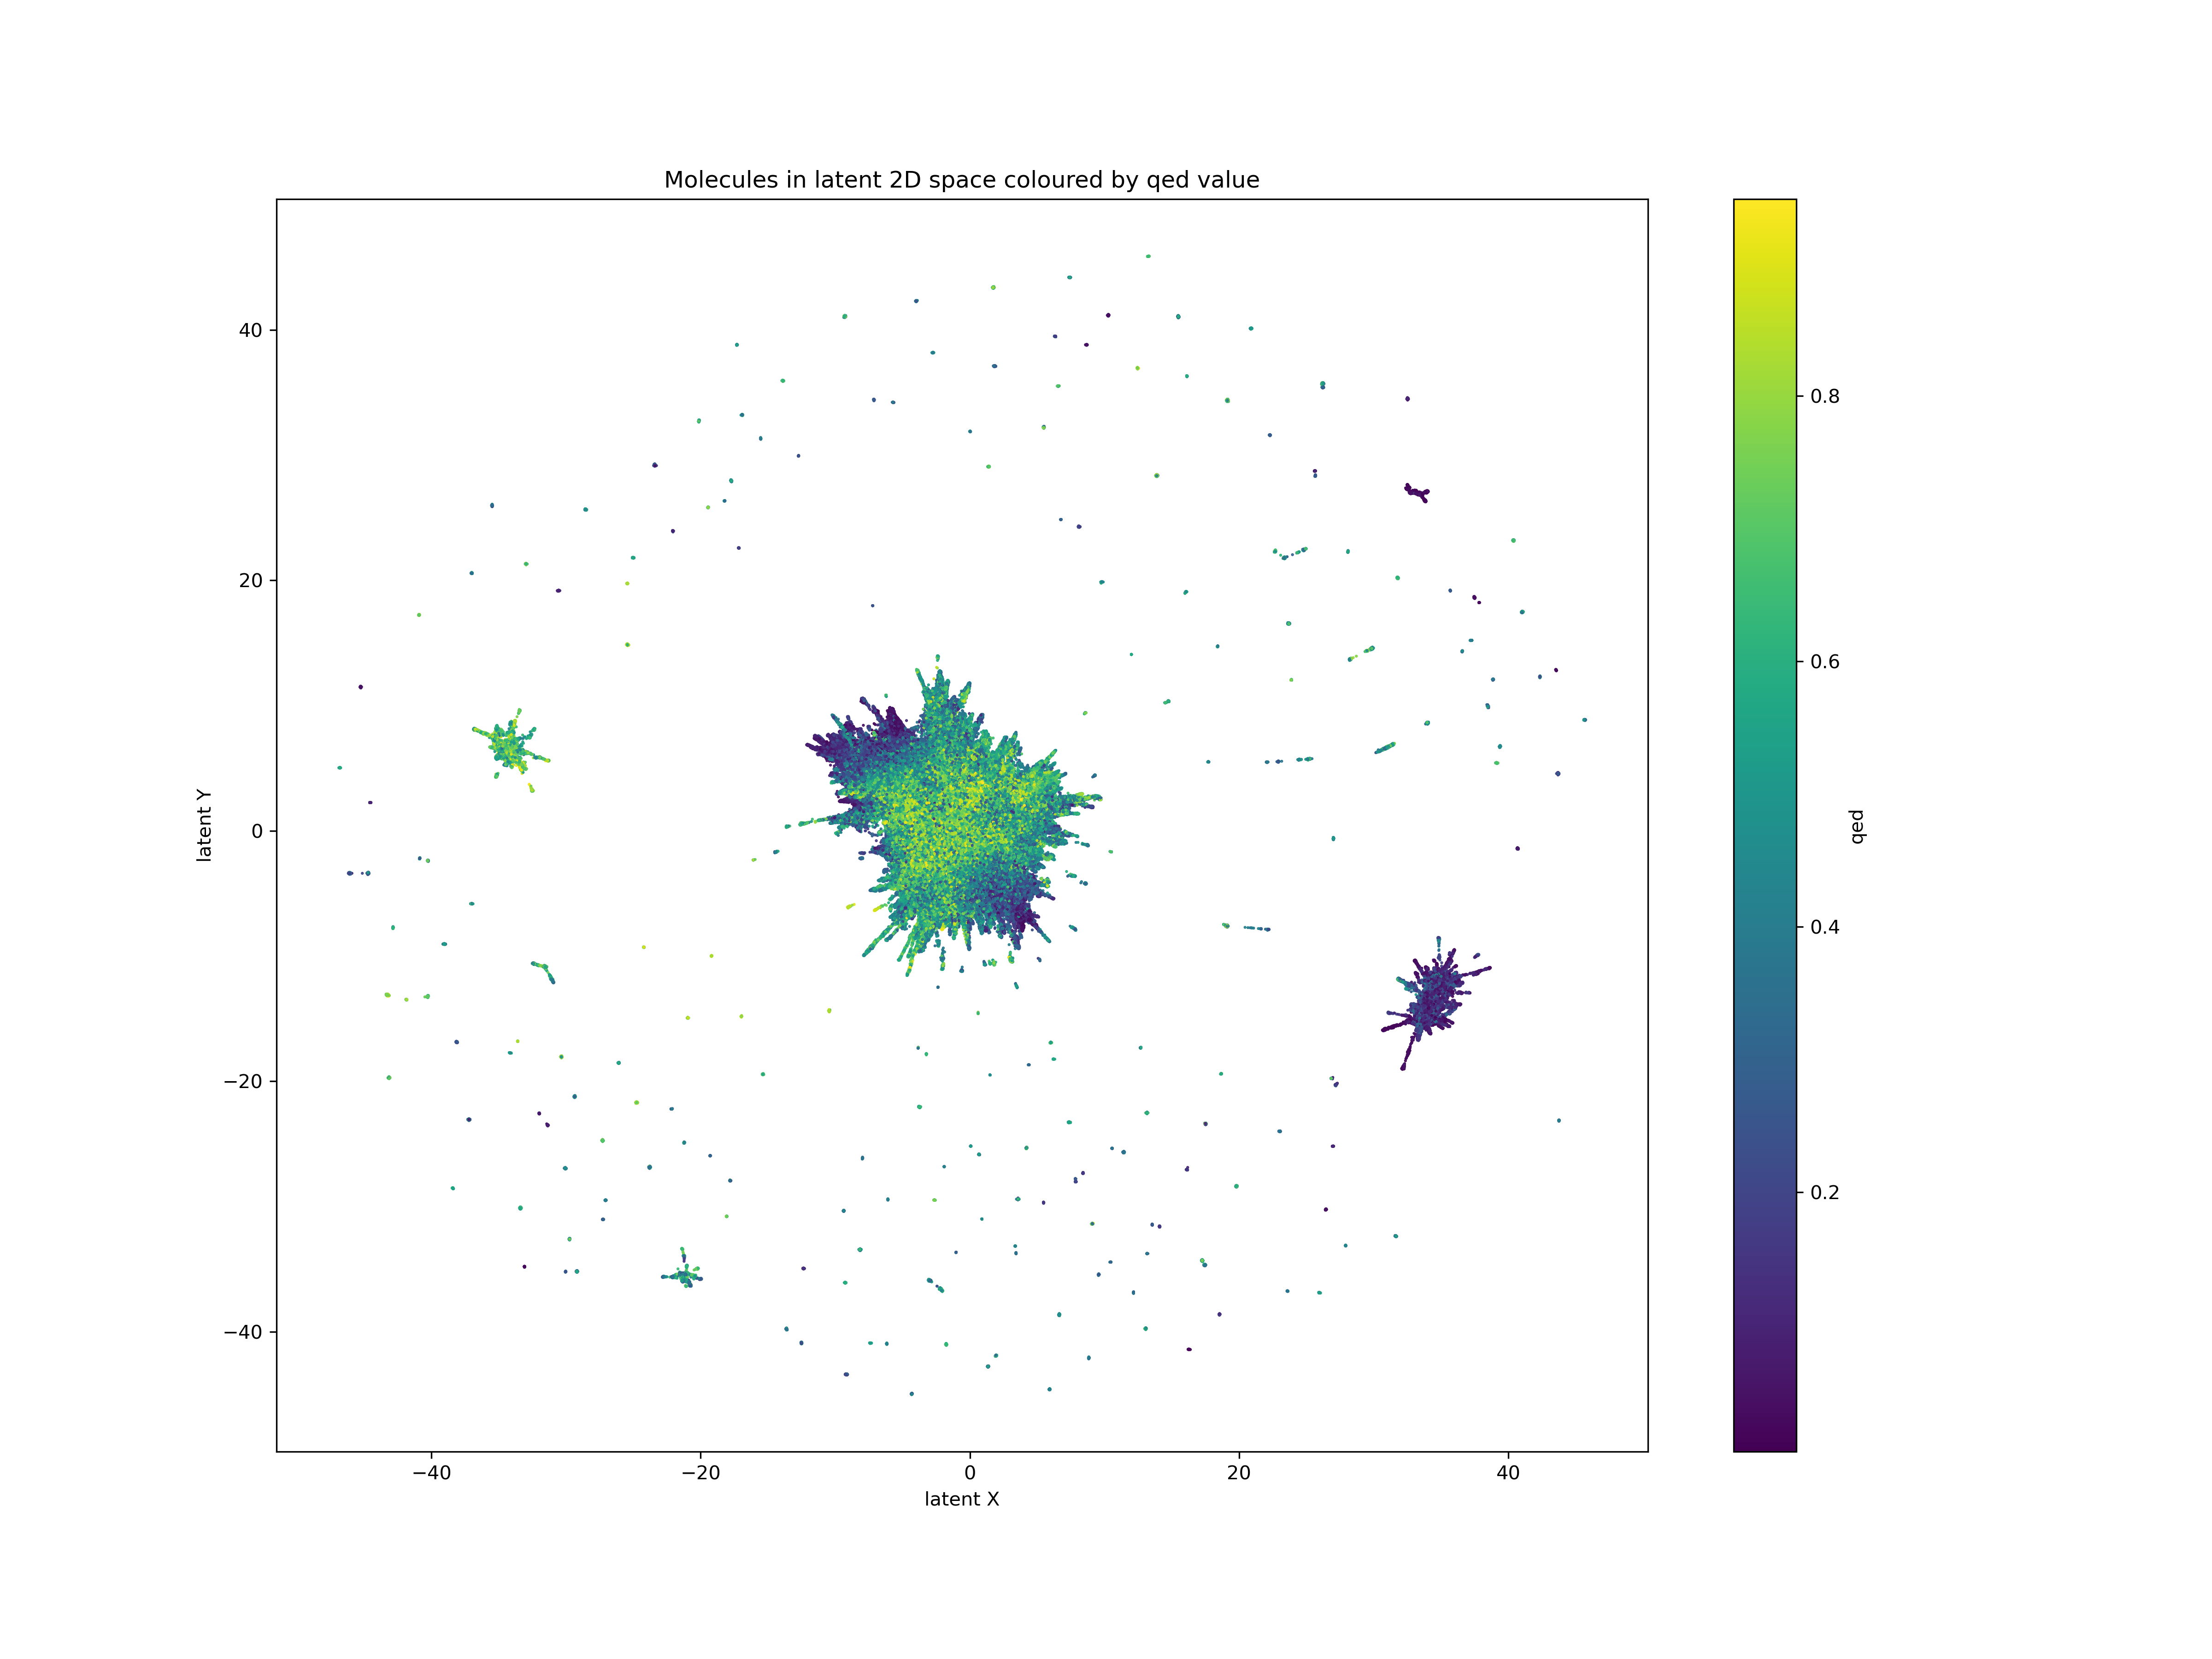
\includegraphics[width=0.49\columnwidth, keepaspectratio]{figures/PaCMAP_default}
	\caption{Results of PCA, t-SNE (sklearn and tsnecuda), UMAP, TriMAP and PaCMAP algorithms on the dataset with default parameters, coloured by the quantitative estimate of drug-likeness of each data point. It can be clearly seen that each algorithm places points very differently.}
	\label{fig:default_run}
\end{figure}

The choice of descriptors matter because different metrics relate differently to chemical structure. For example, the melting point of a substance is affected mostly by the secondary bonds it can form. Consider \textit{ethane} and \textit{ethanol}. These two molecules are structurally very similar, only differing by one oxygen atom. This however changes the strongest secondary bond that can form between individual molecules. While solid ethane is bound together only by \textit{van der Waals forces}~\cite{bib:vanderwaals}, solid ethanol is held together by \textit{hydrogen bonds}~\cite{bib:hbond}, many times stronger. As such, while the melting point of ethane is $-182.8~^\circ$C, ethanol melts at $-114.14~^\circ$C. The difference is even more dramatic for boiling points, $-88.5~^\circ$C and $+78.23~^\circ$C for ethane and ethanol respectively.

The ideal descriptors are those that do not change very much as the structure of molecules changes a little. In the end, I chose the following metrics: Quantitative estimate of drug-likeness, Ring count, number of hydrogen donors, number of hydrogen acceptors, topological polar surface area~\cite{bib:tpsa} and number of rotatable bonds.

It should be noted that some of these descriptors do jump slightly from molecule to molecule, however, this change is not too great to cause problems in interpreting data.


As can be seen on figure (\ref{fig:default_run}), the different algorithms yielded in substantially different embeddings. This is a direct result of the differences highlighted in table (\ref{tab:graph}). 

PCA produces the smoothest transition. This might seem positive, but in reality, this is not ideal. Chemical descriptors, qed in particular are not monotonous over chemical structure. This means that similar while similar molecules have similar qed values, dissimilar molecules might have the exact same qed. For this reason, a complete gradient is undesirable. This stems from the fact that PCA performs a linear transformation, not allowing for the preservation of such structures.

Another interesting thing is the difference in sklearn t-SNE and tsnecuda (second and third graph respectively). The sklearn implementation did not differentiate dissimilar points into distinct clusters. Investigating this phenomenon lead to the discovery that sklearn's implementation was bugged, only iterating for a mere 150 iteration, which was not enough for separation of different molecules, as can be seen on figure (\ref{fig:tsne:iter_sweep}). t-SNE has the most uniform clustering in terms of density of points among the graph-based algorithms. It should be noted that t-SNE did not use the default perplexity value, as I have found previously that a perplexity parameter of around 1000 produces the most desirable output. 

UMAP clusters the molecules in one big cluster (although not as extremely as PaCMAP), with a few little clusters on the side. This is partly due to the low default min\_dist parameter, making ultra-tightly packed clusters. The space is very much smooth over qed value. 

TriMAP creates objects resembling magnetic field lines. This is very interesting from a structural view. It should be noted however, that it seems like the individual clusters overlap with each other in a way that no other algorithm resembles. For this reason, targeted search would be very difficult on a space created by TriMAP. This particular problem as we will see does not get better with tuning parameters, making TriMAP fundamentally unusable for this use-case.

PaCMAP -- similarly to UMAP -- produces one compact cluster in the middle, with some additional clusters nearby. This behaviour is not ideal for targeted search, since quite different molecules are placed near each other. PaCMAP does offer very much control over its sightedness however, and with different parameters, this can change.

Overall, with default parameters, it initially seems like t-SNE produces the most desirable embedding. TriMAP resulted in the least useful output space out of the graph-based algorithms. This will however change with other parameters, as the values are tuned to represent the dataset faithfully.

\section{Optimizing the parameters}\label{sec:optimizing-the-parameters}

As discussed previously, an advantage of parametrizable algorithms is the fact that the user is able to influence the preservation of local or global structure according to their use-case. For optimal results, each algorithm was run multiple times with different parametrization. The choice of parameters to sweep was based on how much effect it had theoretically. 

\subsection{t-SNE}

There are many common parameters of graph-based algorithms, mainly because of the use of gradient descent. Indeed, the effect of these parameters do not have significantly different effects with other methods. Because of this, I will only present the parameters associated with GD with t-SNE.

The optimization of gradient descent is in and of itself a vast topic worth many books. In fact, many papers have been written on this very topic. The graph-based algorithms all use gradient descent and all have some form of optimization laid out in their respective original papers. For this reason, the only parameter I will show now is the number of iterations. This is one of the most important parameters of gradient descent as too few iterations will inevitably prevent the convergence on a local minimum, while too many iterations needlessly increases the runtime of the algorithm and can even lead to overfitting, the production of an analysis that corresponds too closely or exactly to a particular set of data, and may therefore fail to fit additional data or predict future observations reliably.

\begin{figure}[!h]
	\centering
	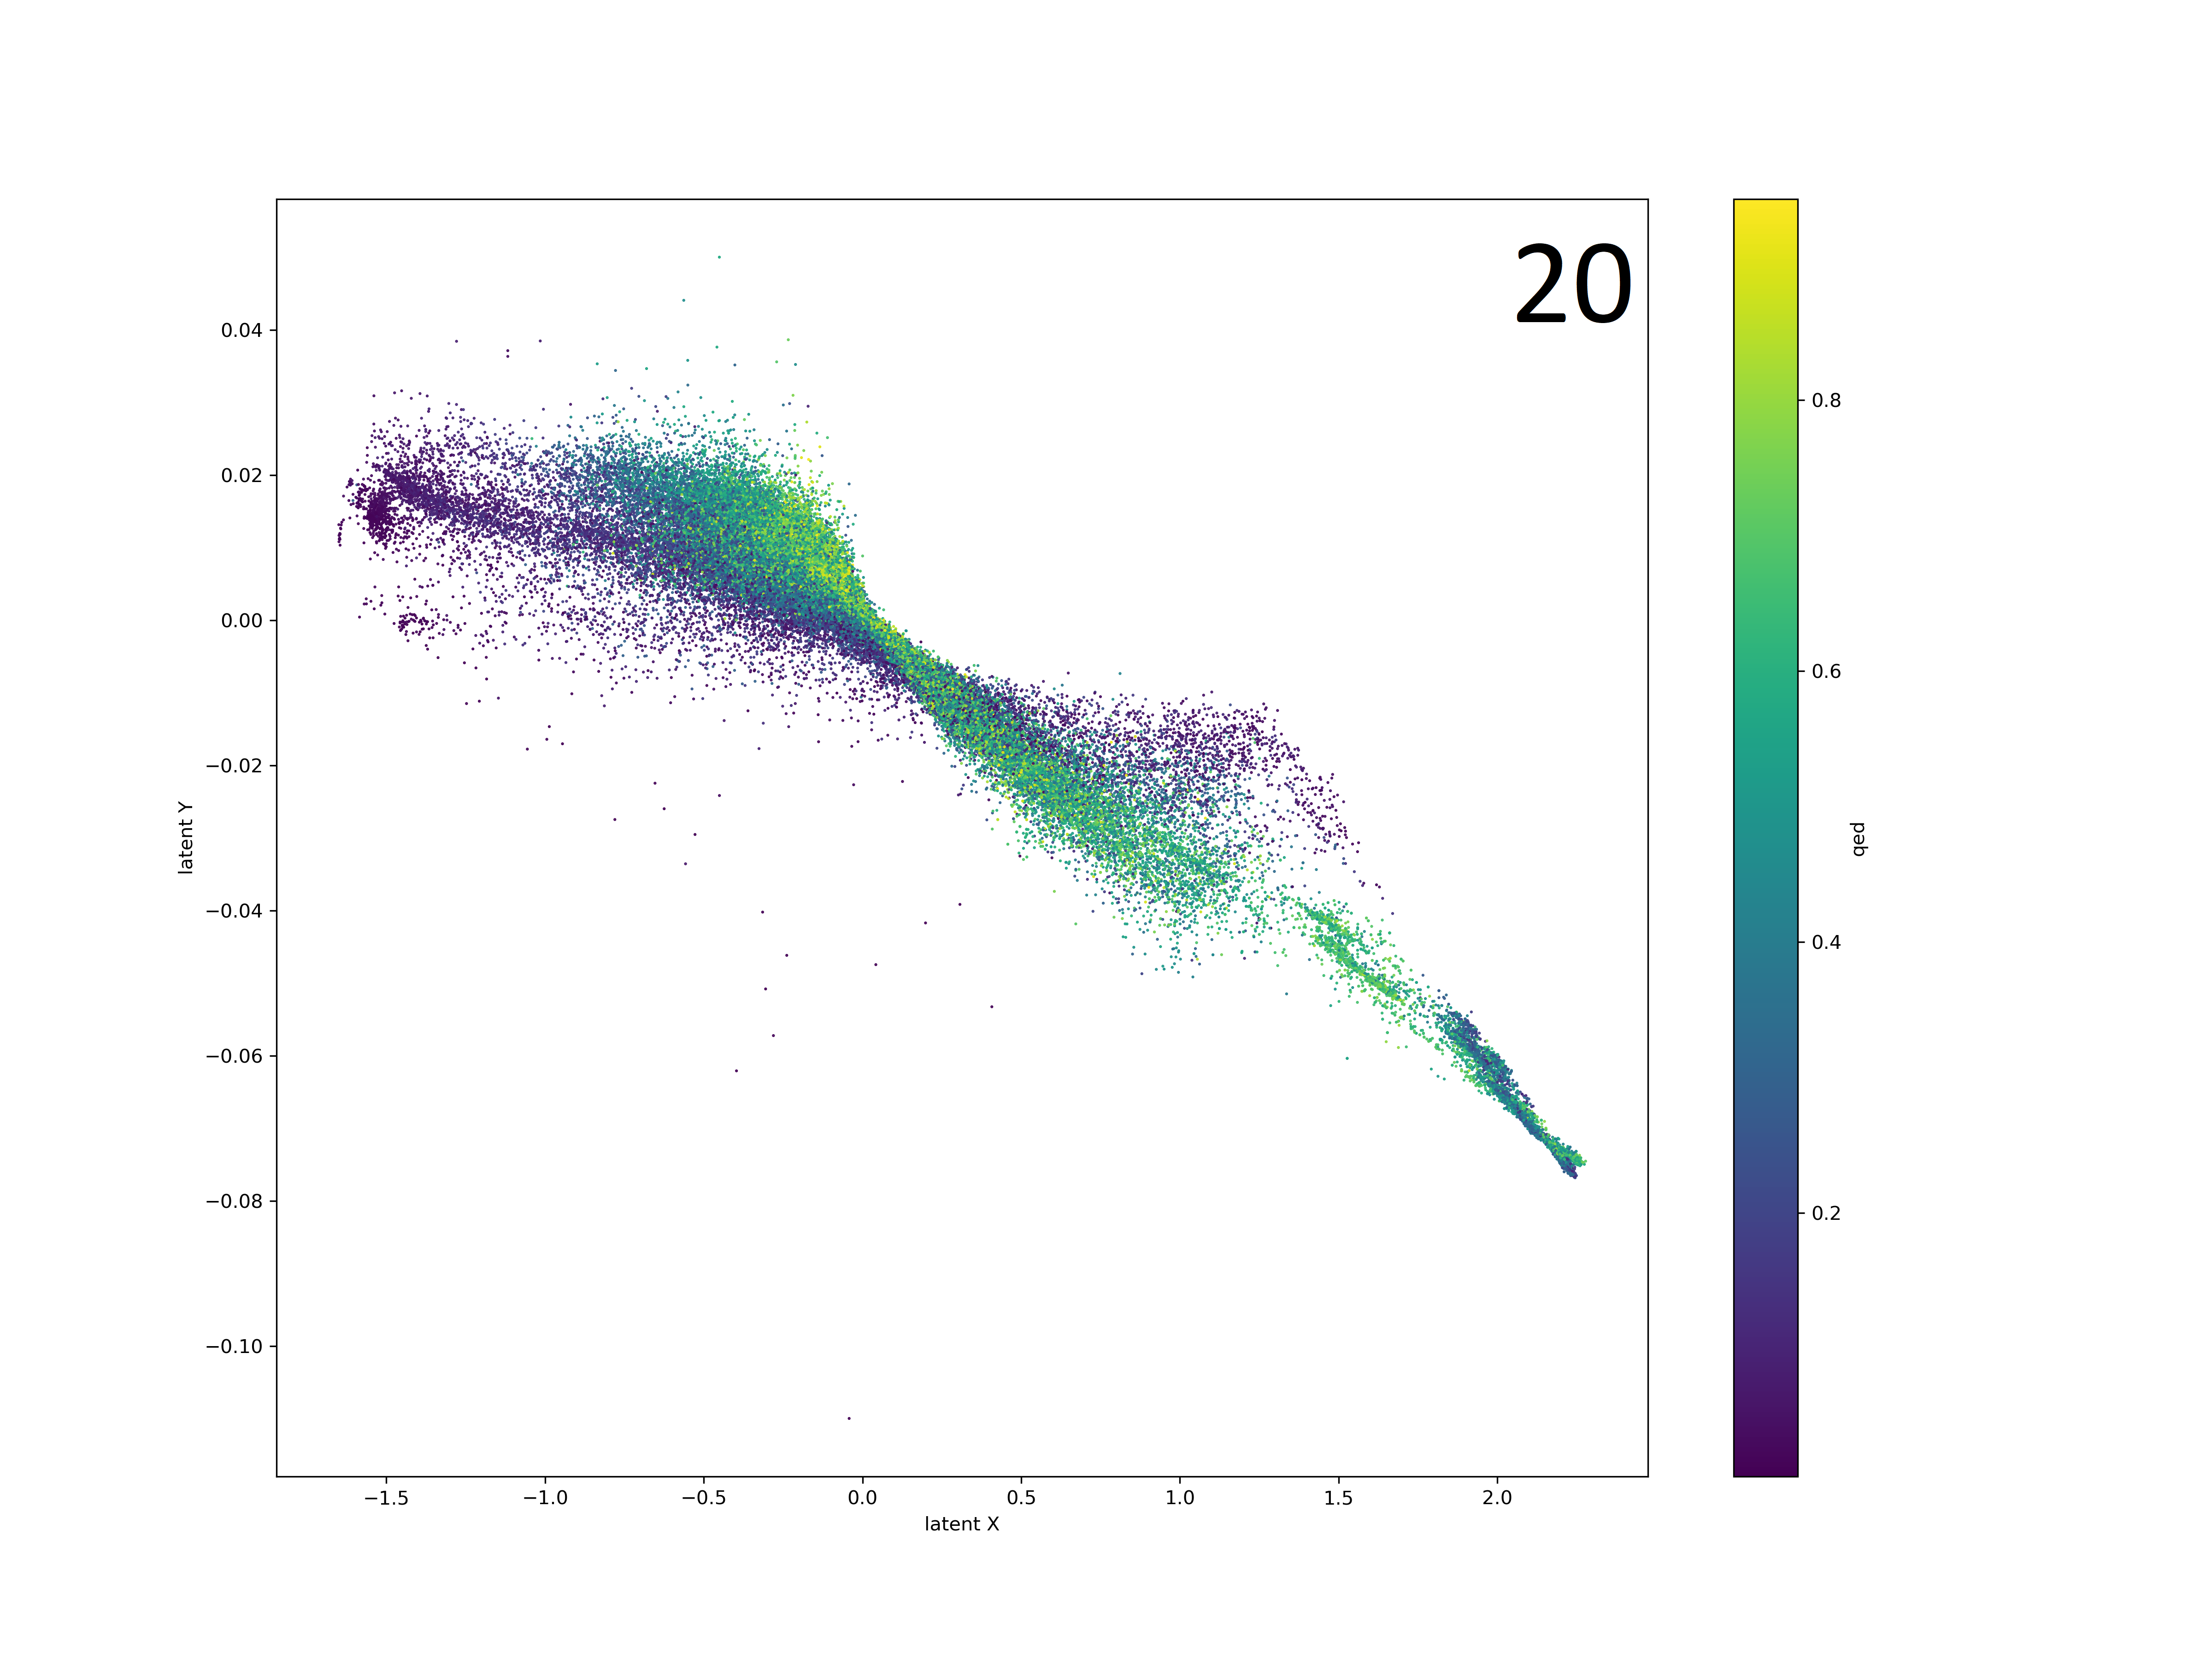
\includegraphics[scale=0.1]{figures/qed20iter}
	\includegraphics[scale=0.1]{figures/qed50iter}
	\includegraphics[scale=0.1]{figures/qed200iter}
	\includegraphics[scale=0.1]{figures/qed500iter}
	\includegraphics[scale=0.1]{figures/qed1000iter}
	\caption{Result of the same t-SNE run after 20, 50, 200, 500 and 1000 iterations. The initial closeness of points comes from early exaggeration during gradient descent. It can be clearly seen that initial iterations change the embedding significantly, while later iterations only have minor effects.}
	\label{fig:tsne:iter_sweep}
\end{figure}

The effect of n\_iters does not scale linearly. In the initial iterations, the gradient of the error surface tends to be large, meaning that every step has a significant effect on the overall embedding. As the iterations go on however, the output approaches a local minimum, changing less and less every step. This effect is demonstrated by figure (\ref{fig:tsne:iter_sweep}), where in the first few hundred iterations significant change can be seen, while during the last 500 iterations only minor differences arise.

The most important parameter of t-SNE is perplexity. As described in section (\ref{sec:t-sne}), perplexity affects the $\sigma_i$ used in equation~\eqref{eq:tsne:pi|j}. This parameter is responsible for the focus between local and global structure preservation. This focus shift is rather limited in t-SNE, as figure (\ref{fig:tsne:perplexity}) shows.

\begin{figure}[!h]
	\centering
	\includegraphics[width=0.3\columnwidth]{figures/tsne_qed50perpl}
	\includegraphics[width=0.3\columnwidth]{figures/tsne_qed450perpl}
	\includegraphics[width=0.3\columnwidth]{figures/tsne_qed700perpl}
	\caption{Effect of perplexity on t-SNE. The values 50, 450 and 700 were used on a subset ($n = 100000$) of the whole database. Even significantly different perplexity values generate similar embeddings.}
	\label{fig:tsne:perplexity}
\end{figure}

It seems like this parameter does not have a large effect on the result. This can be attributed to the fact that perplexity does not directly affect the algorithm, only indirectly. Because of this, using the perplexity parameter does not allow fine control over the resulting embedding. It is possible that even higher, more extreme values of perplexity have more desirable effects, however, the memory consumption of $k$-nearest neighbour search for larger values of $k$ -- which is indirectly being increased with high perplexity -- renders it practically unusable.

\subsection{UMAP}


UMAP has two particularly interesting parameters when it comes to the result of the embedding. These are min\_dist and n\_neighbours. The former dictates the minimum distance between points that are in the same cluster, while the latter is the number of nearest neighbours searched for in the initial stage of the algorithm. 

The first parameter, min\_dist has a very drastic effect on the embedding. With low values of min\_dist, clusters there is no penality for placing intra-cluster points very closely, forming  highly compact clusters. This also means that different clusters are separated more clearly. With higher values, even points in the same cluster are placed further apart, making a more uniform distribution of points, that have less cluster separation. This effect is shown on figure (\ref{fig:umap:min_dist}). 

\begin{figure}[!h]
	\centering
	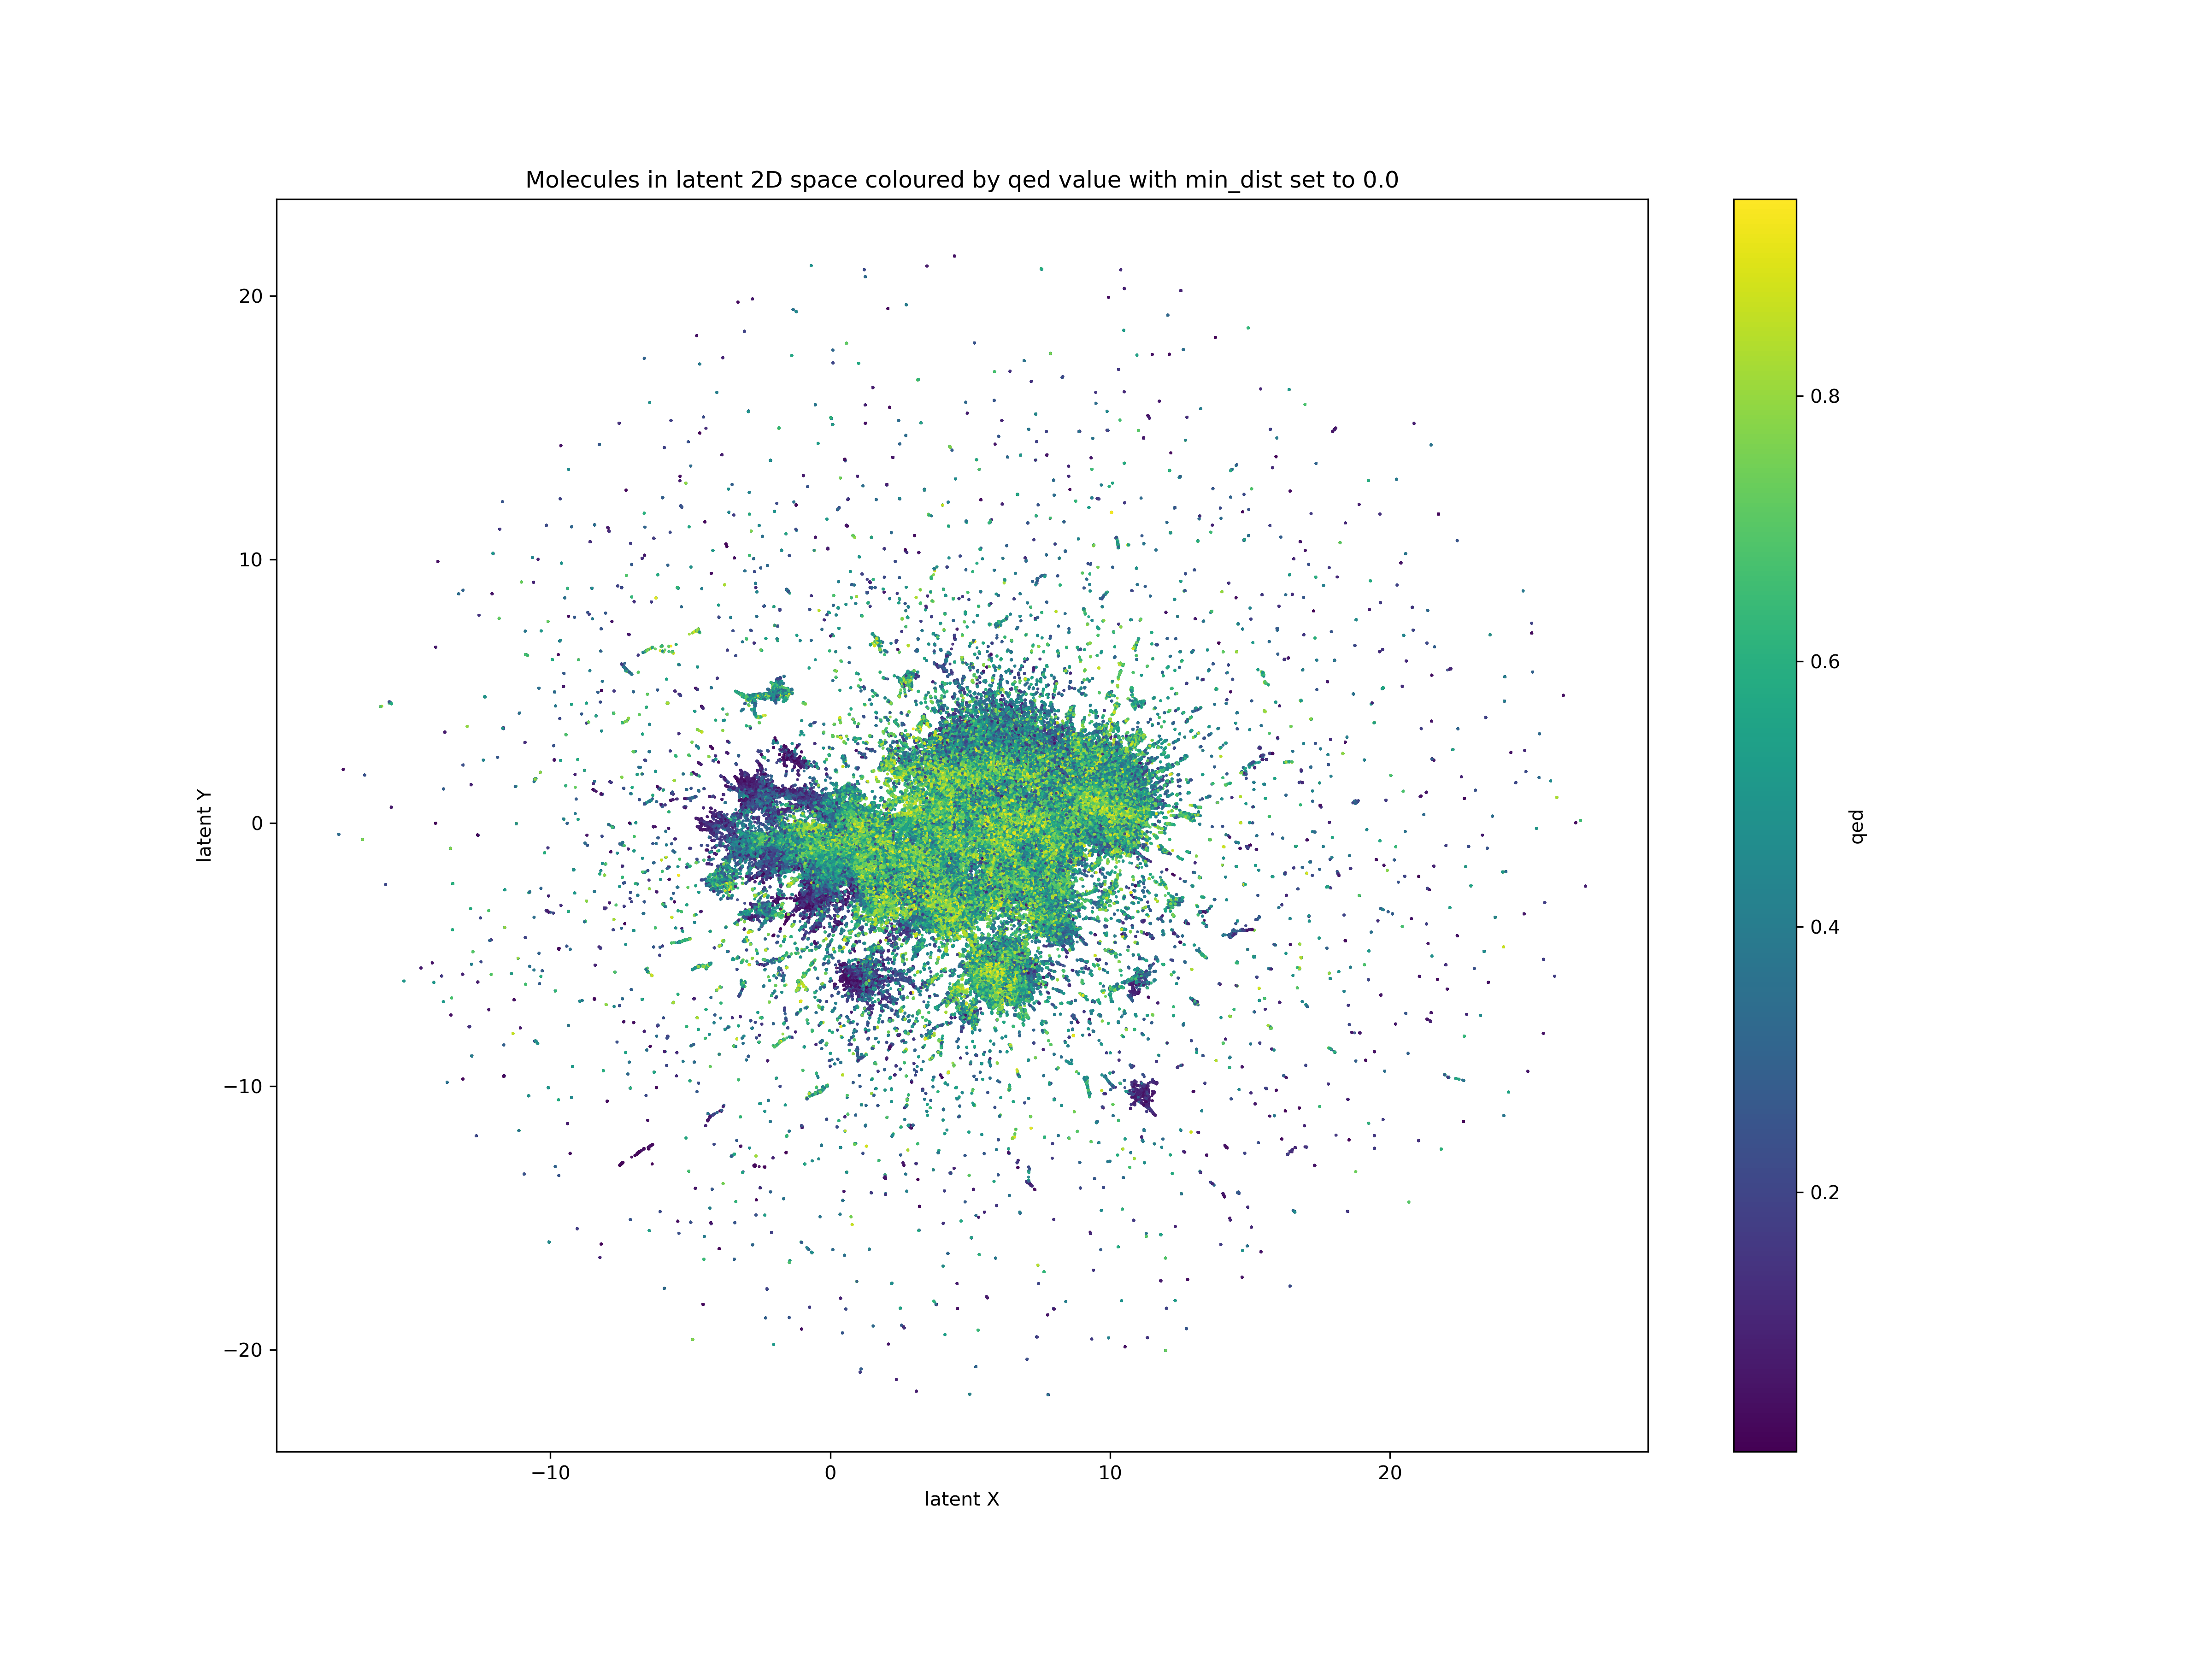
\includegraphics[width=0.32\columnwidth]{figures/UMAP0.0}
	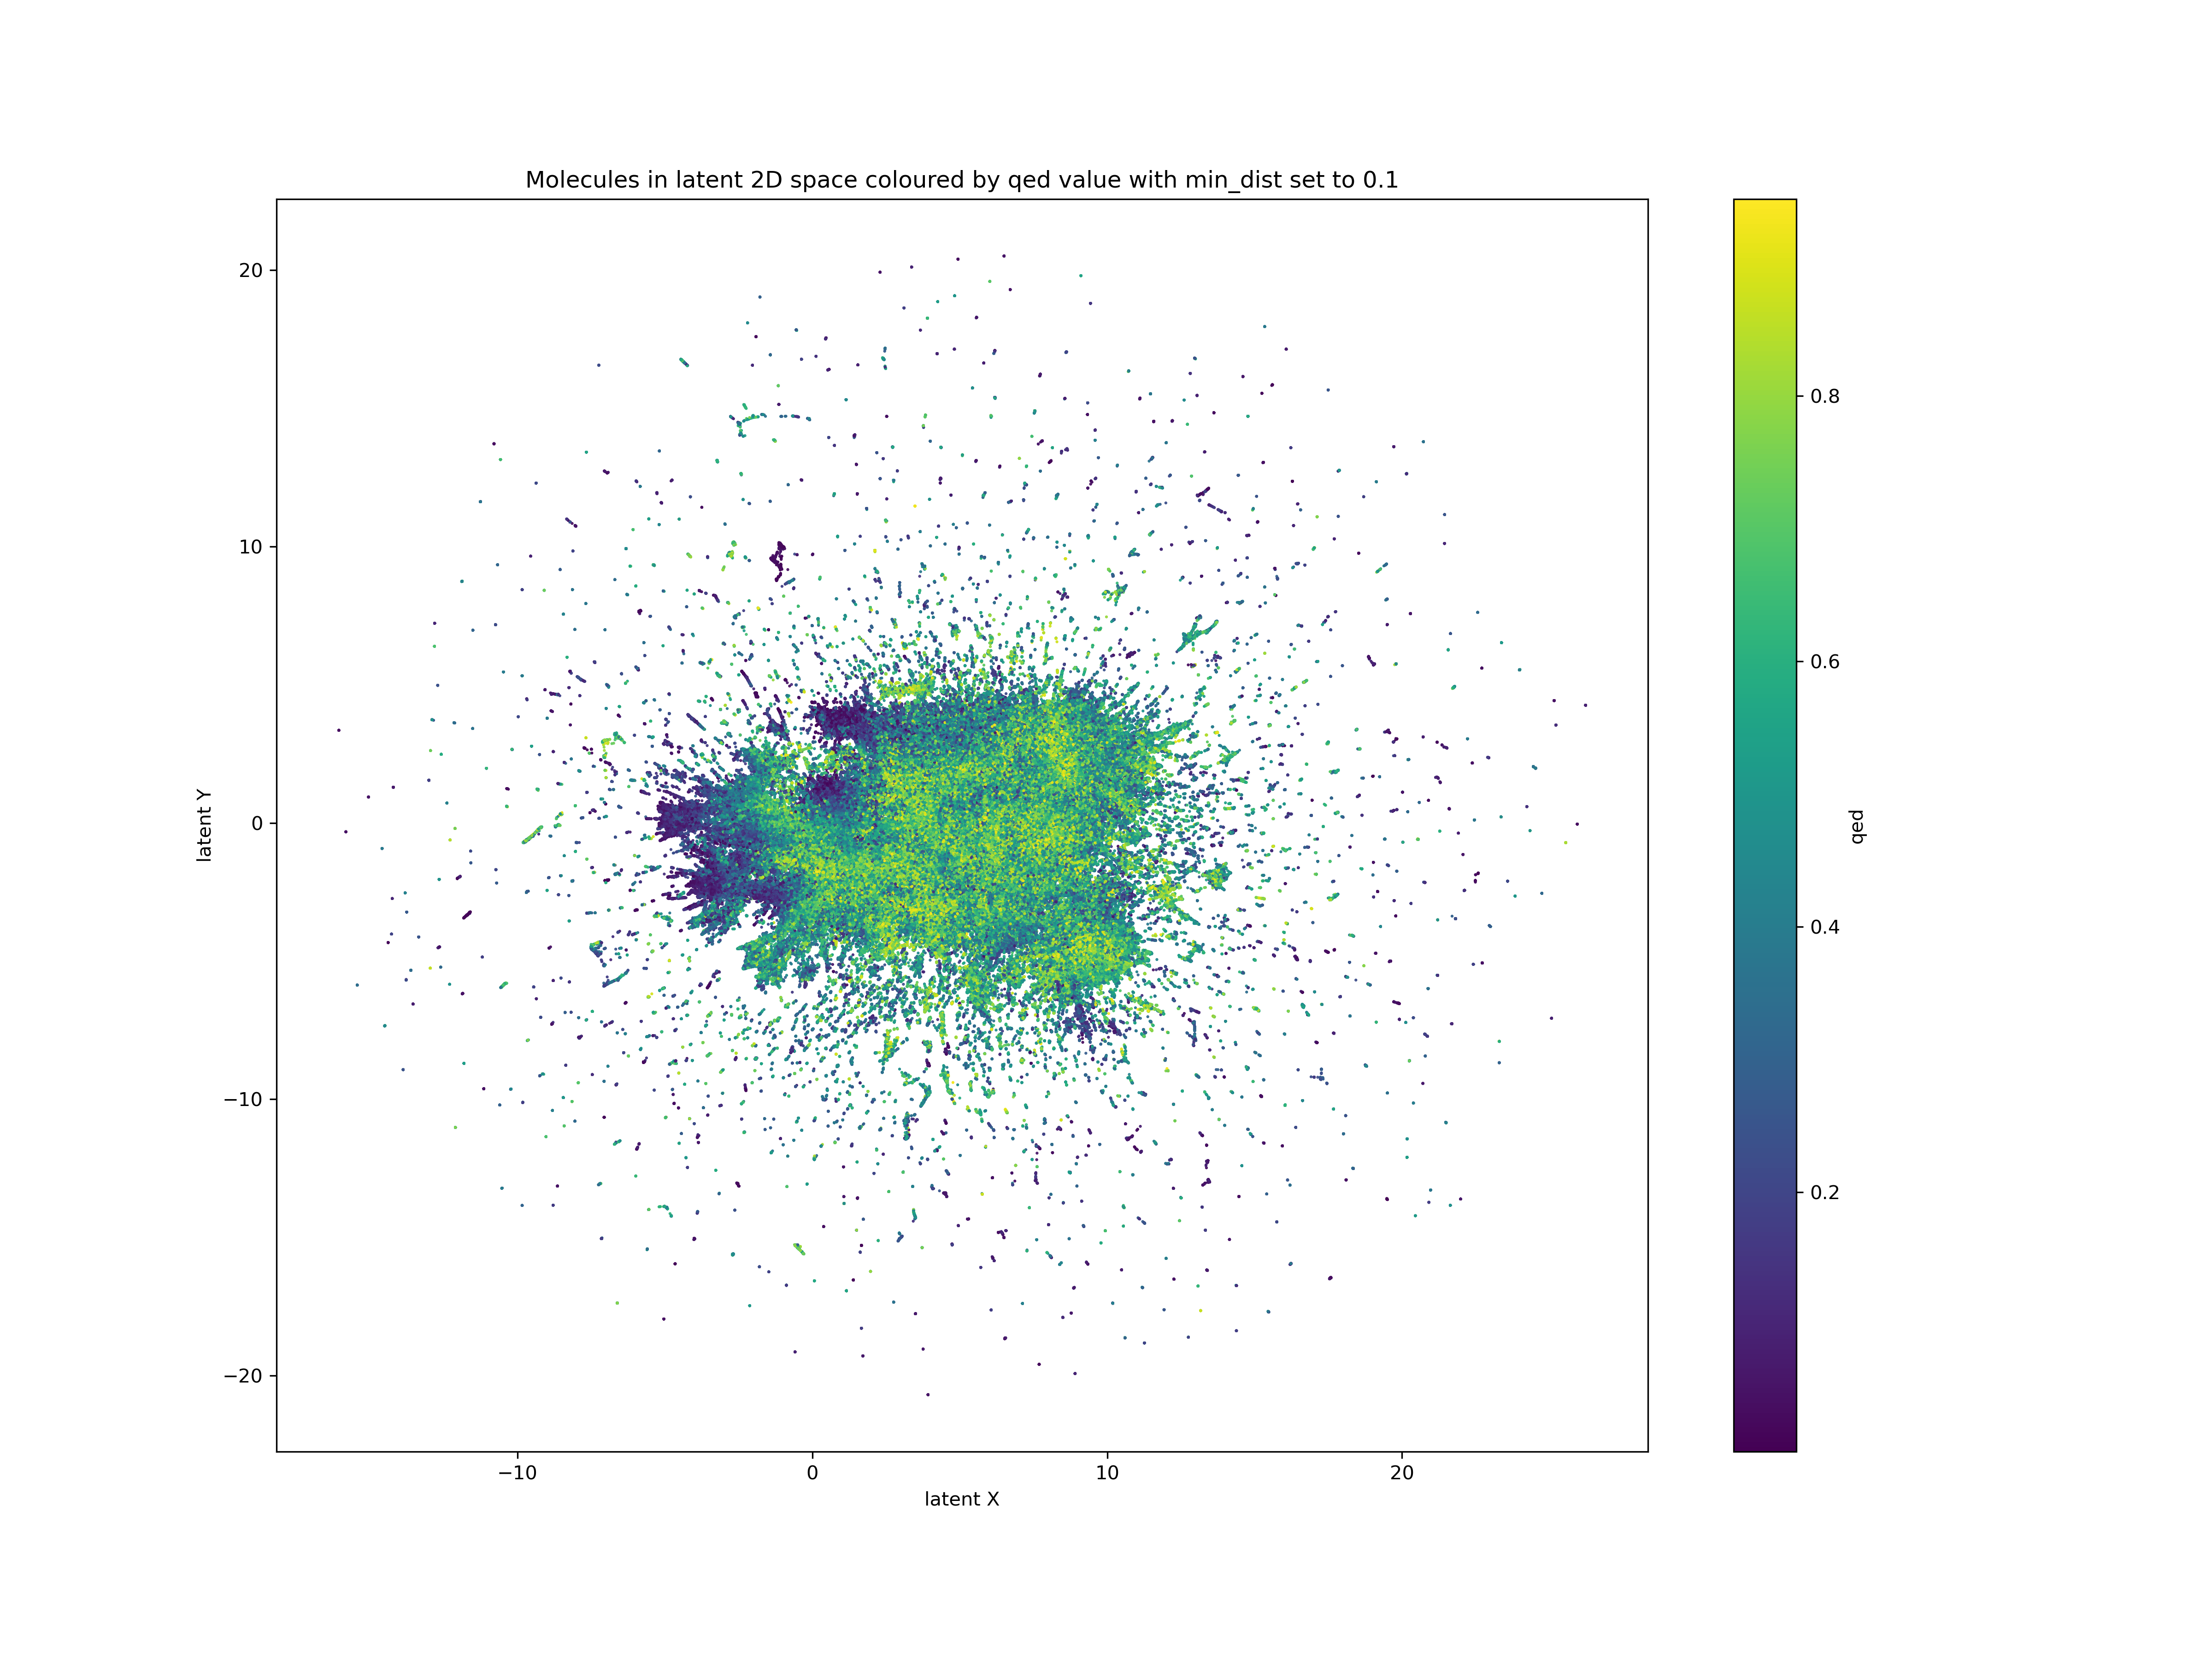
\includegraphics[width=0.32\columnwidth]{figures/UMAP0.1}
	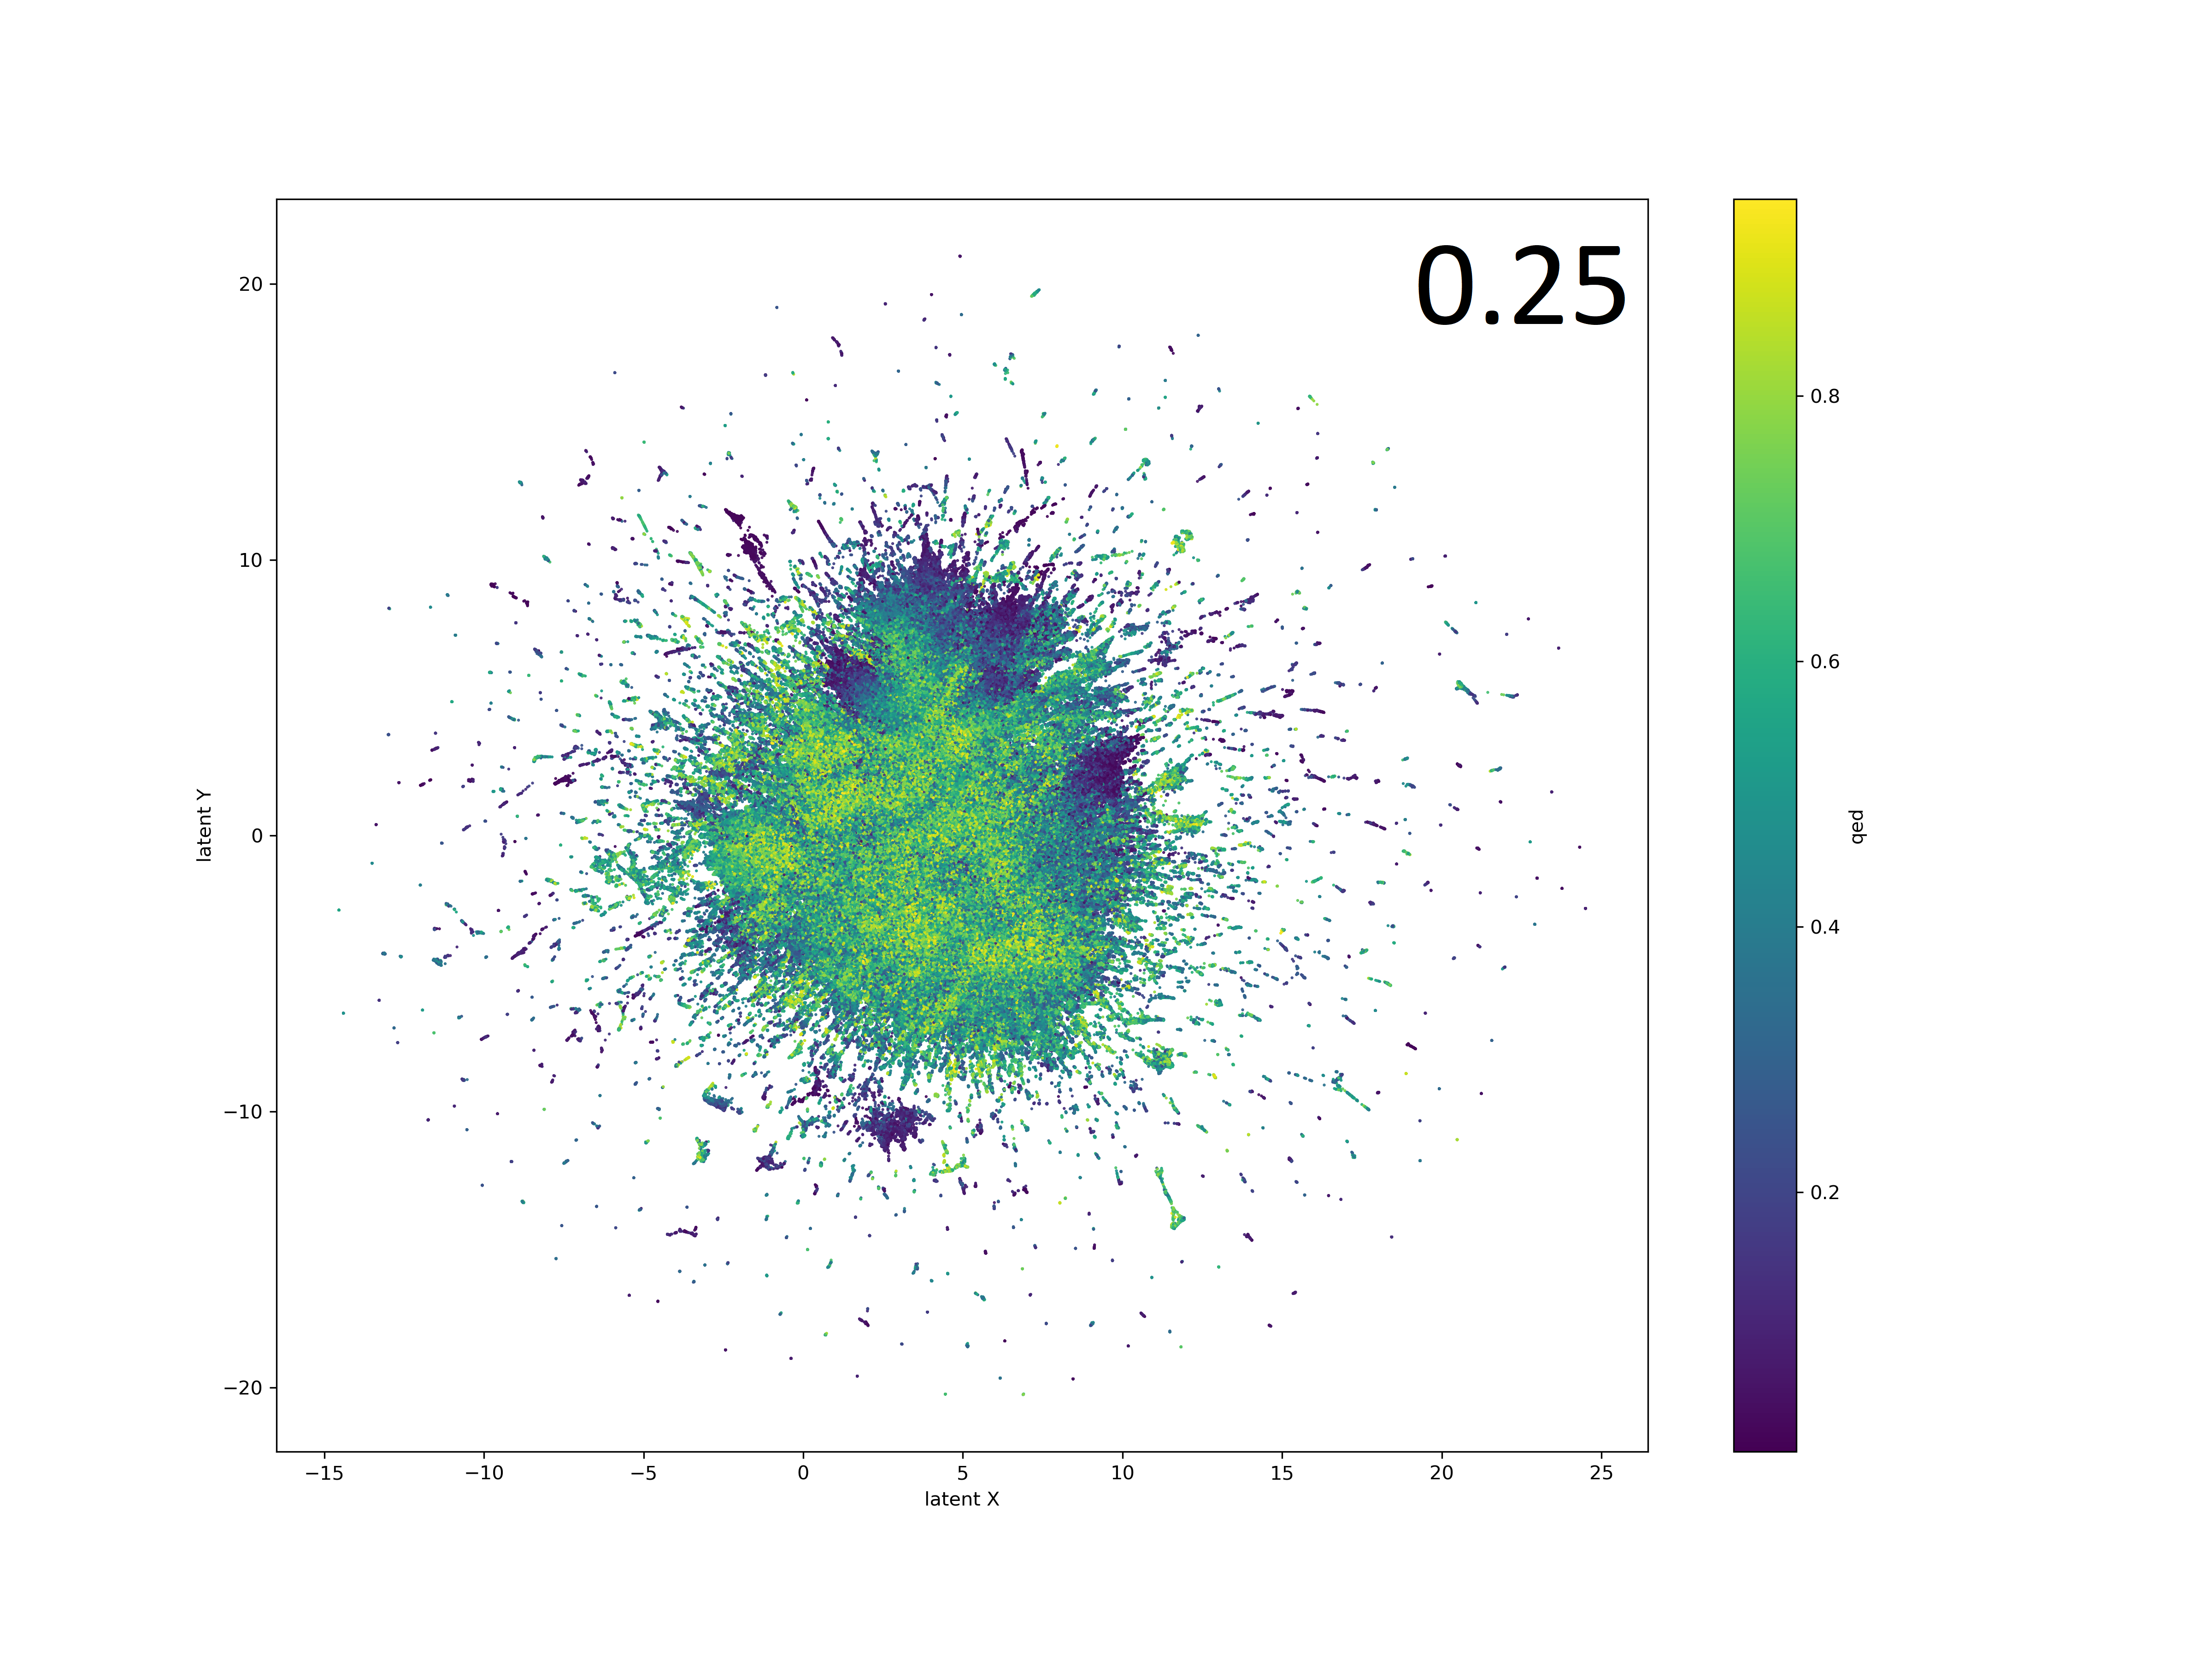
\includegraphics[width=0.32\columnwidth]{figures/UMAP0.25}
	\includegraphics[width=0.32\columnwidth]{figures/UMAP0.5}
	\includegraphics[width=0.32\columnwidth]{figures/UMAP0.75}
	\includegraphics[width=0.32\columnwidth]{figures/UMAP0.99}
	\caption{Effect of min\_dist parameter on the embedding produced by UMAP. The values are in order: 0.0, 0.1, 0.25, 0.5, 0.75 and 0.99. As the value increases, so does the space between points in the same cluster, making the whole space more spread out.}
	\label{fig:umap:min_dist}
\end{figure}

While the ultra-tight clusters allow more separation of inter-cluster molecules, for the purpose of targeted search, they are undesirable. This is due to the fact that in tightly-packed clusters, sampling must be done very closely to the original point, meaning even small changes in the location of a sampled point can result in very different chemicals. This however can be solved by generating the low min\_dist embedding and scaling every point too. The major drawback of such a procedure is that targeted searching in the scaled space results in scaled points that have to be rescaled for further use. 

While the exact optimum of this parameter is not objectively measurable, according to figure (\ref{fig:umap:min_dist}) a value of around 0.75 seems to be the sweet spot for balance between tightly packed clusters and uniformly placing the molecules. 

The number of nearest neighbours is the parameter of UMAP that shifts the focus from local to global structure. With a larger number of nearest neighbours, a more global structure is approximated in the initial stage of UMAP. This in turn results in the lower dimensional graph being optimized for more global structure preservation. 

\begin{figure}[!h]
	\centering
	\includegraphics[width=0.32\columnwidth]{figures/UMAP@0.75@10}
	\includegraphics[width=0.32\columnwidth]{figures/UMAP@0.75@30}
	\includegraphics[width=0.32\columnwidth]{figures/UMAP@0.75@50}
	\includegraphics[width=0.32\columnwidth]{figures/UMAP@0.75@100}
	\includegraphics[width=0.32\columnwidth]{figures/UMAP@0.75@200}
	\caption{Effect of n\_neighbours parameter at values of 10, 20, 30, 50, 100, 200 with a min\_dist parameter of 0.75. Higher values result in more compact overall embedding, as more and more points are counted as nearest neighbours. At particularly high values (such as 200), very few distinct clusters are formed and all molecules are placed on top of each other just like with TriMAP.}
	\label{fig:umap:n_neighbor}
\end{figure}

As can bee seen on figure (\ref{fig:umap:n_neighbor}), the value of n\_neighbours has a drastic effect when changed from a low value to a slightly higher one, however, at larger values the difference in embedding starts to diminish. One interesting thing that can be seen on is the gradual disappearance of clusters in favour of a uniform blob. For targeted searching, this is potentially bad, since so many molecules are packed into one space. For this reason, very high values are undesirable for this use-case.

\subsection{TriMAP}

\begin{itemize}
	\item n\_inliers are the most important parameter
	\item very small effect on actual embedding
\end{itemize}

\subsection{PaCMAP}

\begin{itemize}
	\item most important parameter is FP\_ratio
	\item it forces PaCMAP to preserve local structure
	\item very significant effect on result
	\item time of embedding is very dependent on this parameter
\end{itemize}

\begin{itemize}
	\item UMAP and PaCMAP improved most
	\item PaCMAP has most potential for good embedding, UMAP closely follows
\end{itemize}

\section{Overall results of hyperparameter optimization}\label{sec:overall-results-of-hyperparameter-optimization}


\section{Linear interpolation test}\label{sec:linear-interpolation-test}

\begin{itemize}
	\item important for targeted search
	\item between similar molecules and random ones
	\item only 100 points to not screw up embedding
	\item optimally a line is drawn  between ends
	\item PCA made straight line, not surprising
	\item t-SNE split points into two clusters
	\item UMAP traced the path between them
	\item also has run where they aren't so far away
	\item TriMAP places new points very far away
	\item PaCMAP makes proper line
	\item with random points, it splits points into two clusters
	\item also has run where they are in one cluster
	\item UMAP has most promising results
\end{itemize}

\begin{figure}[!h]
	\centering
	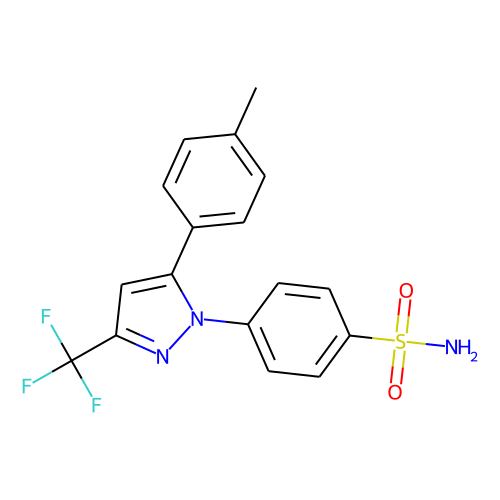
\includegraphics[width=0.4\columnwidth]{figures/coxib1}
	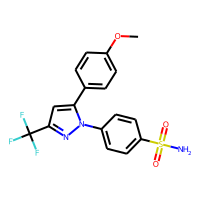
\includegraphics[width=0.4\columnwidth]{figures/coxib2}
	\caption{Two similar molecules (0.742 Tanimoto similarity) used in the linear interpolation test. The one on the left is celecoxib, a well-known COX-2 inhibitor. }
	\label{fig:coxib}
\end{figure}

\begin{figure}[!h]
	\centering
	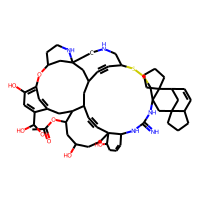
\includegraphics[width=0.4\columnwidth]{figures/random_mol1}
	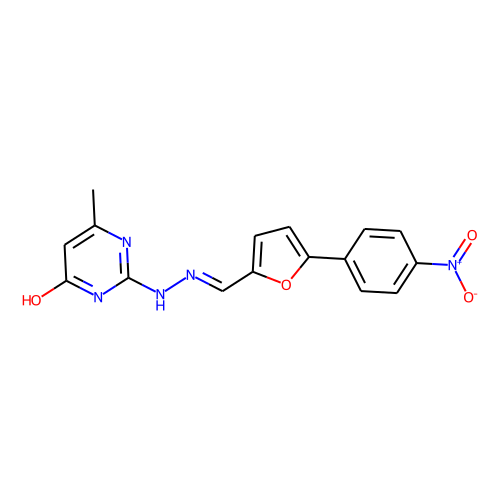
\includegraphics[width=0.4\columnwidth]{figures/random_mol2}
	\caption{Two randomly selected molecules that were used in the linear interpolation test. The two molecules have very distinctly different structures, and as such belong in different clusters.}
	\label{fig:random_mol}
\end{figure}